\documentclass{article}
\usepackage[utf8]{inputenc}
\usepackage{amsmath}
\usepackage{amssymb}
\usepackage{graphicx}
\usepackage{algorithm}
\usepackage[noend]{algpseudocode}
\usepackage{hyperref}
\usepackage{xcolor}

\hypersetup{
    colorlinks=true,
    linkbordercolor = {white},
    linkcolor=black,
    urlcolor=cyan
}
\title{Problème de clique maximum}

\author{Drissi Mohamed Reda}

\begin{document}

\maketitle
\newpage
\tableofcontents
\newpage
\section{Introduction}
Nous prenons un graphe $G=\{V,E\}$ tel que $V$ est l'ensemble des sommets
et $E$ l'ensemble des arrêtes(Nous ignorons les arrêtes liant une arrête à elle même). \\
Nous nommons les sommets du graphe 1,2, ... n. Cet algorithme permet de trouver une clique
de taille d'au moins $k$. À chaque étape, si nous trouvons une clique de taille d'au moins
$k$, nous arrêtons.
\section{Algorithme et Test}
\subsection{Algorithme}
\begin{algorithm}
\begin{algorithmic}
  \Function{Expand\_clique}{Graph Q}
  \While{$\exists$ v joignable à Q}
    \State trouver $v_{max}$ tel que Le nombre de sommets joignable à la clique $Q \cup \{v_{max}\}$ est maximal
    \State $Q \gets Q\cup \{v_{max}\}$
  \EndWhile
    \State \Return $Q$
  \EndFunction
\end{algorithmic}
\end{algorithm}
\begin{algorithm}
\begin{algorithmic}
  \Function{Alter\_Clique}{Graph Q}
  \State Trouver $v \notin Q$ tel que $\exists! w \in Q$ non adjacent à $v$.
    \If{$v = \varnothing$}
      \State \Return $Q$
    \Else
      \State $Q\gets Q \setminus \{w\}$
      \State $Q \gets Q \cup \{v\}$
      \State $Q \gets$ \Call{Expand\_clique}{Q}
      \State \Return $Q$
    \EndIf
  \EndFunction
\end{algorithmic}
\end{algorithm}

\begin{algorithm}[!htp]
\caption{Algorithme de clique de taille k}
\begin{algorithmic}[1]
  \For{i $\in$ [1,n]}
    \State initialiser la clique $Q_i\gets \{i\}$
    \State $Q_i \gets$ \Call{Expand\_Clique}{$Q_i$}
    \For{i $\in$ [1,k]}
      \State $Q_i \gets$ \Call{Alter\_Clique}{$Q_i$}
    \EndFor
  \EndFor
  \ForAll{$Q_i$ et $Q_j$ trouvés}
    \State initialiser la clique $Q_{i,j} \gets Q_i \cap Q_j$
    \State $Q_{i,j} \gets$ \Call{Expand\_Clique}{$Q_{i,j}$}
    \For{i $\in$ [1,k]}
      \State $Q_i \gets$ \Call{Alter\_Clique}{$Q_i$}
    \EndFor
  \EndFor

\end{algorithmic}
\end{algorithm}
\subsection{Example}
Comme example nous prenons le graphe complémentaire du \href{https://en.wikipedia.org/wiki/Frucht\_graph}{graphe de Frucht}
Avec les sommets :
\begin{displaymath}
  V=\{1,2,3,...12\}
\end{displaymath}
\begin{center}
  \begin{figure}[!htp]
    \caption{Complément du graphe de Frucht}
    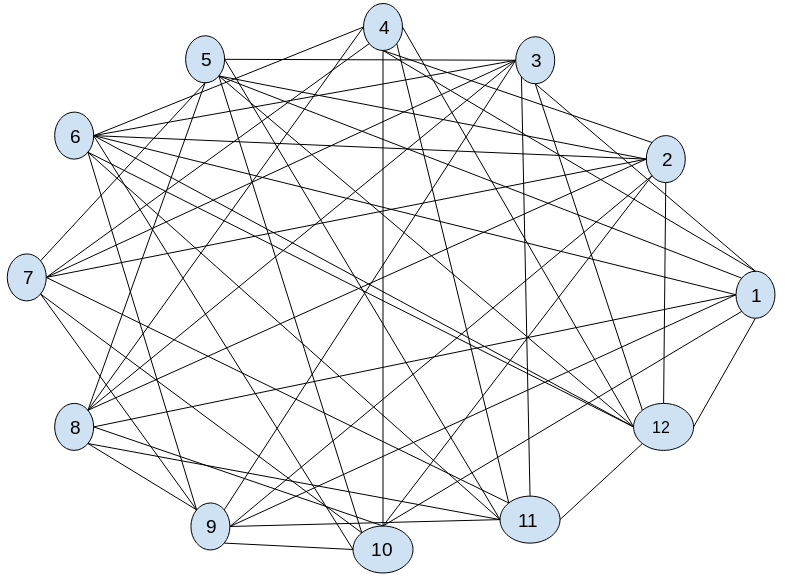
\includegraphics[scale=0.5]{Report/frucht-compl.png}
  \end{figure}
\end{center}

Nous allons faire tourner cet algorithme pour trouver une clique d'au moins $k=5$. \\
Pour i=1 et i=2 nous trouvons des cliques de taille 4 donc nous passons à i=3.
Initialisation : $Q_3=\{i\}=\{3\}$. \\
Nous exécutons la fonction \textit{Expand\_Clique}
\begin{center}
  \begin{tabular}{|c|c|c|}
    \hline
    sommet $v$ joignable à $Q_3$ & sommets joignables à $Q_3\cup\{v\}$ & taille \\ \hline
    \hline
    1 	& 5, 6, 8, 9, 12  	& 5 \\ \hline
    5   & 1, 7, 8, 11, 12   & 5 \\ \hline
    6 	& 1, 9, 11, 12  	  & 4 \\ \hline
    7 	& 5, 9, 11, 12  	  & 4 \\ \hline
    8 	& 1, 5, 9, 11 	    & 4 \\ \hline
    9 	& 1, 6, 7, 8, 11 	  & 5 \\ \hline
    11 	& 5, 6, 7, 8, 9, 12 & 6 \\ \hline
    12 	& 1, 5, 6, 7, 11  	& 5 \\ \hline
  \end{tabular}
\end{center}
Nous trouvons que le maximum est :
\begin{displaymath}
  |Q_3 \cup \{v\}|_{max}=6 \quad pour \quad v=11
\end{displaymath}
Nous ajoutons le sommet $6$ à $Q$. Nous retrouvons la nouvelle clique \\
$Q_3=\{3, 11\}$ de taille 2.
\begin{center}
  \begin{tabular}{|c|c|c|}
    \hline
    sommet $v$ joignable à $Q_3$ & sommets joignables à $Q_3\cup\{v\}$ & taille \\ \hline
    \hline
    5 	& 7, 8, 12 	& 3 \\ \hline
    6 	& 9, 12 	  & 2 \\ \hline
    7 	& 5, 9, 12 	& 3 \\ \hline
    8 	& 5, 9 	    & 2 \\ \hline
    9 	& 6, 7, 8 	& 3 \\ \hline
    12 	& 5, 6, 7 	& 3 \\ \hline
  \end{tabular}
\end{center}
Nous trouvons que le maximum est :
\begin{displaymath}
  |Q_3 \cup \{v\}|_{max}=3 \quad pour \quad v=5
\end{displaymath}
Nous ajoutons le sommet $5$ à $Q$. Nous retrouvons la nouvelle clique \\
$Q_3=\{3, 5, 11\}$ de taille 3.
\begin{center}
  \begin{tabular}{|c|c|c|}
    \hline
    sommet $v$ joignable à $Q_3$ & sommets joignables à $Q_3\cup\{v\}$ & taille \\ \hline
    \hline
    7 	& 12 	            & 1 \\ \hline
    8 	& $ \varnothing$ 	& 0 \\ \hline
    12 	& 7 	            & 1 \\ \hline
  \end{tabular}
\end{center}
Nous trouvons que le maximum est :
\begin{displaymath}
  |Q_3 \cup \{v\}|_{max}=1 \quad pour \quad v=7
\end{displaymath}
Nous ajoutons le sommet $12$ à $Q$. Nous retrouvons la nouvelle clique \\
$Q_3=\{3, 5, 7, 11\}$ de taille 4.
\begin{center}
  \begin{tabular}{|c|c|c|}
    \hline
    sommet $v$ joignable à $Q_3$ & sommets joignables à $Q_3\cup\{v\}$ & taille \\ \hline
    \hline
    12    & $\varnothing$ & 0 \\ \hline
  \end{tabular}
\end{center}
Nous trouvons que le maximum est :
\begin{displaymath}
  |Q_3 \cup \{v\}|_{max}=0 \quad pour \quad v=12
\end{displaymath}
Nous ajoutons le sommet $12$ à $Q$. Nous retrouvons la nouvelle clique \\
$Q_3=\{3, 5, 7, 11, 12\}$ de taille 5.\\
Puisque la clique est de taille 5, nous nous arrêtons là.
\section{Complexité}
Nous allons calculer la complexité de cet algorithme :
Nous allons supposer les cas les plus pessimistes, bien que ça ne soit impossible pour en arriver
à ce genre de situations, la plupart des cas testés trouvent un résultat dans la fonction
\textit{find\_cliques} sans passer à \textit{pairwise\_intersections}.\\
Soit $G$ un graphe ayant $n$ sommets et une clique $Q$ :
\subsection{complexité de \textit{add\_vertex}}
La fonction \textit{adjoinable} prend au pire $n^2$ itérations donc une compléxité de $O(n^2)$.
Car chaque sommet moins de $n$ sommets qui ne sont pas voisins, et cela prends $n$ itérations pour
vérifier si un sommet non voisin ne fait pas partie de la clique.\\
Pour chaque clique, trouver le nombre de sommets joignables prends au pire $n$ fois la fonction
\textit{adjoinable}, ce qui en résulte que la complexité de la fonction \textit{max\_adjoinable} est
de $O(n^3)$.\\
Puis pour chaque clique trouver qu'un sommet où le nombre de sommets joignables est maximal prends
$n$ fois la fonction \textit{max\_adjoinable}, puisqu'il y a au pire, $n$ sommets en dehors de la
clique, donc $n*O(n^3)=O(n^4)$. La fonction \textit{add\_vertex} s'achève si au pire $n$ sommets
ont été ajoutés à la clique donc nous trouvons $n*O(n^4)=O(n^5)$.\\
La complexité de \textit{add\_vertex} est de $O(n^5)$.
\subsection{Complexité de \textit{expand\_vertex}}
Pour trouver un sommet $v \notin Q$ qui a exactement un sommet $w \in Q$ qui n'est pas son voisin
nous avons besoin d'au pire $n^2$ itérations. Si nous trouvons un tel sommet $w$ nous avons besoin
d'une seule itération.\\ Puis nous avons besoin de $O(n^5)$ pour performer \textit{add\_vertex}.\\
La complexité de \textit{expand\_vertex} est donc de $O(n^5)$.
\subsection{Complexité de \textit{find\_cliques}}
Pour chaque itération, \textit{add\_vertex} prends $O(n^5)$ puis \textit{expand\_vertex} est exécutée
au pire $n$ fois (puisque $k \leq n$). Alors la complexité est de $O(n^5+n*n^5)=O(n^6)$. \\
Puisqu'on exécute ces itérations $n$ fois, alors la complexité devient :
\begin{displaymath}
  O(n*n^6)=O(n^7)
\end{displaymath}
\subsection{Complexité de \textit{pairwise\_intersections}}
Nous avons moins de $n^2$ de paires distinctes de cliques maximales trouvées par \textit{find\_cliques}
Donc similairement à \textit{find\_cliques} pour chaque itération la complexité sera de $O(n^5+n*n^5)=O(n^6)$
exécutée $n^2$ fois, cela donne $n^2*O(n^6)=O(n^8)$.
\subsection{Complexité totale}
La complexité totale sera la somme de la complexité de \textit{find\_cliques}, \textit{find\_neighbors}
et \textit{pairwise\_intersections}. Donc :
\begin{displaymath}
C(n)=O(n^2)+O(n^7)+O(n^8)
\end{displaymath}

\section{Implémentation}
Nous implémentons en C++ l'algorithme trouvé précédemment pour trouver la clique
maximum d'un graphe.

\section{Test}
Nous allons faire tourner notre code C++ sur plusieurs graphes, notre algorithme
nous permet de choisir la taille de la clique souhaitée, cela rends le code plus partique
pour s'assurer de trouver la clique maximale, nous allons choisir un nombre n=k
Ce graphe :
\begin{center}
  \begin{verbatim}
    0 0 0 1 0 0 1
    0 0 0 0 1 0 1
    0 0 0 0 0 1 1
    1 0 0 0 1 1 0
    0 1 0 1 0 1 0
    0 0 1 1 1 0 0
    1 1 1 0 0 0 0
  \end{verbatim}
\end{center}
donne le résultat :
\begin{center}
  \begin{verbatim}
  1. Clique of size 3 : 4 5 6
  \end{verbatim}
\end{center}
Passons aux choses sérieuses, nous avons téléchargé des graphes en format \texttt{.clq.b} depuis les
instances de \href{https://cse.unl.edu/~tnguyen/npbenchmarks/clique.html}{DIMAC}. \\
Avant de passer aux tests il faut expliquer l'arborescence des fichiers.
\begin{itemize}
  \item \textbf{bingraph:} Contient les graphes téléchargés depuis le site en \texttt{.clq}.
  \item \textbf{edgls:} Contient les listes d'arrêtes de chaque graphe en \texttt{.ls} convertie avec \texttt{bin2asc}
    obtenu depuis \href{https://cse.unl.edu/~tnguyen/npbenchmarks/instances/converter.tar.gz}{ce site}.
  \item \textbf{adjmat:} Contient les matrices d'adjacences en \texttt{.mat}obtenues avec \texttt{edgtoadj}
  \item \textbf{outclq:} Contient les cliques résultantes en \texttt{.out}.
\end{itemize}
Nous pouvons obtenir le graphe sous différentes formes depuis les dossiers précédemment mentionnés.\\
\textbf{N.B:} Nous allons compiler en mode non verbose (par défaut) pour ne retenir que les informations
importantes, le détail sera à consulter depuis les \texttt{.out}.
\paragraph{Keller4}
Commande :
\begin{verbatim}
time ./clique keller4 11
\end{verbatim}
Résultat
\begin{verbatim}
  Graph keller4
  Graph has n = 171 vertices.
  Find a Clique of size at least k = 11
  Finding Cliques...
  Found Clique of size at least 11.
  Results are stored in outclq/keller4.out file
\end{verbatim}
Temps d'exécution :
\begin{verbatim}
  real	0m0.036s
  user	0m0.032s
  sys	  0m0.000s
\end{verbatim}
\end{document}
